%%%%%%%%%%%%%%%%%%%%%%%%%%%%
% Mini Proposal
% Spring 2016
% Snow distribution on glaciers
%%%%%%%%%%%%%%%%%%%%%%%%%%%%

\documentclass[12pt]{article}
\usepackage[letterpaper, margin=1in]{geometry}
\usepackage{graphicx}
\usepackage{natbib}
\usepackage{wrapfig}
\usepackage{caption}
\usepackage{subcaption}
\usepackage{multirow}
\usepackage[table,xcdraw]{xcolor}
\usepackage{subfig}

\begin{document}

\title{Snow distribution on glaciers}
\author{Alexandra Pulwicki \\ Earth Science SFU}
\date{\today}
\maketitle

\section{Introduction}

\begin{wrapfigure}{R}{0.5\textwidth}
 \centering
      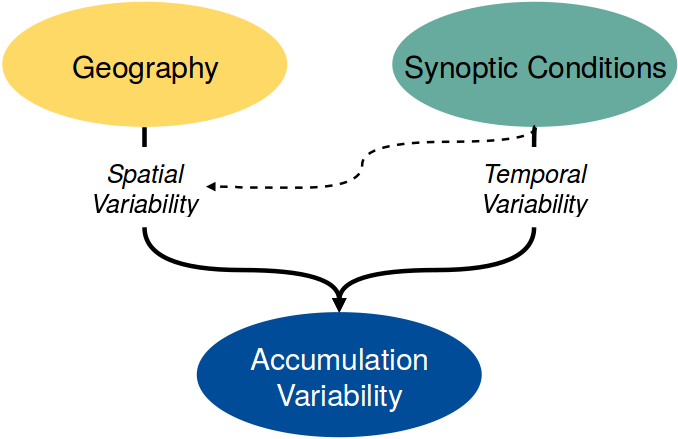
\includegraphics[width=0.5\textwidth]{flow1.png}
  \caption{Interactions between geographic and synoptic conditions contribute to accumulation variability}
	\label{flow1}
\end{wrapfigure}

Snow accumulation, as the dominant input of mass to alpine glaciers, plays an important role in governing their mass balance and the hydrology of alpine catchments more broadly. This has implications not only for the availability of water for local ecological and human uses \citep{ONeel2014,Barnett2005}, but also for rates of global sea-level rise \citep{Gardner2013}. It is therefore critical to thoroughly understand the spatial distribution of snow on glaciers. Achieving such an understanding however is complicated by the fact that snow distribution in alpine regions is not uniform or static, but rather highly variable and influenced by diverse and dynamic processes operating on multiple spatial and temporal scales. Although previous research has attempted to account for these processes through the development of various techniques of measurement and modelling, little is known about how they operate in glacierized alpine environments. This severely limits possibilities of quantifying and predicting snow distribution on glaciers, particularly in remote locations where frequent empirical measurements are difficult \citep{Nolan2015}.

The spatial distribution of snow accumulation can vary significantly. This is a result of interactions between spatially and temporally variable atmospheric conditions and heterogeneous topography (Figure \ref{flow1}) \citep{Deems2006, Liston2006}. Snow accumulation is spatially variable on a number of scales, as described in Table \ref{scale}. The features and conditions that lead to variability at these scales differ and their relative importance depends on the topography and climate of the study area. Inclusion of parameters that describe relevant processes at multiple scales has been shown to improve models that aim to explain measured snow distribution \citep{Marchand2005, Clark2011}. 

\begin{table}[]
\centering
\caption{Relevant spatial scales for snow variability on glaciers. Information from \cite{Clark2011}.}
\label{scale}
\begin{tabular}{lll}
\textbf{Scale} & \textbf{Length} & \textbf{Associated glacier feature}                     \\ \hline
Point          & $<$5 m         & Crevasses, rocks                                               \\
Hillslope      & 1--100 m        & Curvature, slope, local ridges and depressions, avalanching        \\
Watershed      & 100--10,000 m   & Elevation (orographic lifting and freezing level), aspect (shading)                                       \\
Regional       & 10--1000 km     & Horizontal precipitation gradient across mountain range (rain shadow)
\end{tabular}
\end{table}

Snow drift and preferential deposition are crucial process that alter snow distribution  \citep{Winstral2002,Mott2008, Lehning2008,Clark2011} and have been observed to significantly affect accumulation in glacierized basins \citep[e.g.][]{Dadic2010}.  For example, enhanced accumulation has been observed in alpine environments at the point-scale in small depressions and on lee sides of obstacles, on the hillslope scale on the lee side of ridges, and at the watershed scale on sheltered aspects \citep{Harrison1986, Bloeschl1992, Mott2008, Winstral2002, Clark2011}. 

Temporal variability of accumulation is often driven by meteorological conditions. The snow pack evolves over the course of the winter as accumulation events and wind redistribution occur. Inter-annual differences in accumulation are often observed and can be related to the frequency of storms and the presence of certain air masses \citep{Taylor1969}. For example, \cite{Pomeroy1999} found lower accumulation variability in years when wet snow events occurred because the heavier snow limited wind redistribution.

\section{Measuring accumulation}
There are a number of methods that are commonly used to measure accumulation. Snow depth can be measured continuously using ground-penetrating radar (GPR) \citep[e.g.][]{Machguth2006} or digital elevation model (DEM) subtraction \citep[e.g.][]{Deems2006}. These methods have been widely applied but they require expertise in equipment use and data processing, and the cost of using the equipment can be prohibitive. SWE can be measured directly using automated snow pillows, which record the weight of snow that has fallen. These systems are also expensive and require regular maintenance so are typically located in populated areas. \textit{In situ} probing of snow depth and density are simple methods to determine accumulation --- data processing is minimized and field equipment is inexpensive and easy to use. However, these measurements are not continuous and are time consuming to collect. Despite this, direct measurement of snow depth and density are widely-used in snow accumulation studies.

To determine the spatial variability of accumulation, snow density and depth must be measured. To measure bulk density, a column of snow with a known volume is excavated (in a snow pit or with a firn corer) and weighed \citep{Sold2013, Sold2014}. Usually, a number of snow column densities are measured and the average density is taken as representative of glacier-wide density \citep[e.g.][]{Machguth2006, Grunewald2010, McGrath2015}. The most direct way of measuring snow depth is by probing. To determine the snowpack thickness, the height of the snow above the end of the previous year's ablation surface is measured. Usually, a number of snow height measurements are obtained close to each other and the mean value is taken to be representative of that location. For example, \cite{Machguth2006} took the mean of nine snow probe measurements within a 7 m radius as representative of a test site in the ablation zone.  

To determine the glacier-wide SWE, point snow depth measurements from probing need to be extrapolated. This is often done using a statistical regression that accounts for grid cell values of slope, aspect, curvature, and susceptibility to wind redistribution \citep[e.g.][]{Wheler2014,McGrath2015}. A site-specific linear equation is generated and used to predict SWE for each grid cell based on the values of its relevant parameters. 

Temporal changes in snow depth can be measured to provide a time series of snow accumulation, which can be especially useful for identifying large snowfall events (rapid increases in accumulation) and wind erosion (gradual decreases in accumulation). There are a number of methods of measuring SWE with time. Snow depth sensors, such as the SR50, measure changes in distance between the sensor and the snow surface from which SWE can be calculated using an assigned density \citep{Ryan2008}. Multipath modulation of GPS signals can also be used to measure changes in snow height \citep{Larson2009,McCreight2014}. This method allows for the measurement of average snow depth in a $\sim$1000 m$^2$ area around the antenna and an assigned density is then used to find SWE \citep{McCreight2014}.

\section{Statistical Models}
The distribution and variability of a parameter, such as snow water equivalent (SWE), can be estimated using statistical models. These models help to determine relevant processes that affect the distribution of snow, generally by establishing empirical relationships between snow distribution and meteorological and topographic descriptors or conditions. Although no physically-based relations are employed, terrain parameters can act as proxies for processes that are known to occur \citep{McGrath2015}. Inferences made from these models drive the direction of future studies and provide valuable insight into understanding why variability arises.  

Terrain-based parametrization is the linking of geographic parameters determined from terrain modelling and observed conditions. The terrain in the study area is divided into grid cells where terrain parameters (e.g. location, slope, curvature, aspect, ``northness'', wind exposure, topographic similarity) are calculated \citep{Anderson2014,McGrath2015}. The variable of interest is then measured in the study area and a simple statistical relationship between grid-cell terrain parameters and observed data can be established \citep[e.g.][]{Bloschl1991, Liston1998, Anderton2004,McGrath2015}. Multiple linear regressions \citep{Marchand2005, Sold2013, McGrath2015}, parametric probability distributions \citep{Clark2011}, bivariate screening \citep{Anderton2004}, probability distribution functions \citep{Kerr2013}, and regression tree models \citep{Elder1998, Winstral2002, Molotch2005} are among the more popular models. 

Statistical downscaling is the process of determining an empirical relationship between large-scale atmospheric conditions and regional climates \citep{Fowler2007}. These models are trained and validated using gridded reanalysis data from global circulation models (GCMs) and point observations. Performance of these models is measured using correlation coefficients, distance measures (e.g. root mean squared error), or explained variance \citep{Fowler2007}. The simplest model to apply is a regression model, which directly quantifies a relationship between a local variable and a number of large-scale variables. Statistical methods such as multiple linear regressions \citep{Hanssen-Bauer1998}, principal component analysis \citep{Kidson1998}, canonical-correlation analysis \citep{Busuioc2001}, neural networks \citep{Zorita1999}, and singular value decomposition \citep{Widmann2003} can be employed. The large-scale input variables that are usually chosen (e.g. sea-level pressure, geopotential heights) for statistical downscaling are representative of large-scale circulation. 

\section{Snow distribution on glaciers}
While studies of snow distribution in alpine regions are plentiful \citep[and sources within]{Clark2011} there are comparatively few studies on the distribution of snow on glaciers. Although glaciers are often found in alpine environments, they present a different setting for accumulation. The freezing temperatures of glacier ice allow for snow to stick earlier than on the surrounding rocks, which can be above freezing especially in the early part of the accumulation season. Additionally, the surface of a glacier is often less steep than the surrounding peaks, which allows for snow to deposit more easily. The margin of the glacier can also accumulate snow from avalanches released from the surrounding terrain \citep{Bloschl1991, Mott2008}. Further, glaciers do not support vegetation, which has significant effects on snow accumulation in many alpine basins \citep{Pomeroy1999}. Since few studies have been done on this topic, it is difficult to say whether snow distribution on glaciers is fundamentally different than that of an alpine basin. This lack of snow variability quantification points to a significant gap in the literature.

A few studies have measured spatial distribution of glacier accumulation. The earliest accumulation variability studies were conducted in Svalbard by \cite{Winther1998} and later expanded on my \cite{Palli2002} and \cite{Grabiec2011}. Within these studies, considerable variability was observed at all spatial scales. Significant variability was also found between two adjacent glaciers in Switzerland by \cite{Machguth2006}. There was a clear correlation between altitude and snow accumulation on one glacier while the other glacier had no discernible trend, large snow depth fluctuations, and 40$\%$ less accumulation. The most recent and comprehensive study of snow distribution on glaciers was done by \cite{McGrath2015}, which found that SWE was highly variable on hillslope scales and especially large in the ablation area (which has a rough surface due to the presence of crevasses). The dominant control on SWE distribution was altitude, but multiple terrain parameters were needed to capture most of the variance --- after elevation, wind exposure explained the most variance. Additional studies, including \cite{Sold2013}, \cite{Pelt2014}, and \cite{Dadic2010}, also found variability on multiple spatial scales and the need to include many terrain parameters to explain variation. 

Snow data are generally sparse in mountain regions, especially those that are remote \citep{Marcus1970}. The St. Elias Mountains are one such area. These mountains contain the largest non-polar ice field and the longest valley glaciers outside of Greenland and Antarctica \citep{Marcus1970, Danby2003}. Steep climatic gradients across the mountains create sharp changes in glacier cover and mass balance \citep{Clarke2002}. This region currently has the most negative mass budget and is the largest contributor to sea-level rise in the world \citep{Kaser2006, Gardner2013}. Understanding how local glacier mass balance is affected by distribution of snow is therefore critical for accurate predictions of glacier response to a warming climate. 

Research on snow distribution and glacier mass balance in the St. Elias Mountains is limited. Investigation of large-scale accumulation patterns shows that there is a significant difference in accumulation and equilibrium line altitude (ELA) between the marine and continental sides of the mountains \citep{Marcus1970}. \cite{Taylor1969} found that summer precipitation varied on multiple scales and processes such as orographic lifting, frontal movement, and wind speed and direction all contributed to variability. The mass balance (including an accumulation survey) has been measured on a few alpine glaciers in the eastern part of the St. Elias Mountains \citep[e.g.][]{Wheler2014}. The winter balance was determined on these glaciers by recording snow depth at a number of fixed stakes and using a simple multiple linear regression model to find SWE  \citep{Wheler2014}. Snow mass balance in a non-glacierized alpine basin was examined by \cite{Pomeroy1999}. It was found that wind had a significant impact on the distribution of snow and differences in interannual snowfall affected how susceptible it is to wind effects. Sublimation was also identified as a important process in snow loss. 

There is clearly a strong need for a more comprehensive understanding of snow accumulation in the St. Elias Mountains. Although a few studies have examined accumulation, no studies have examined the distribution of snow and how it varies spatially. This is especially true of small alpine glaciers in the St. Elias Mountains, since the majority of accumulation differences have been observed on large glaciers. It is likely that orographic lifting as well as wind redistribution and preferential deposition play major roles in determining accumulation on small alpine glaciers, so future studies should focus on the impact of these factors. 

\section{Proposed Research}

\begin{table}[]
\centering
\caption{Tentative sampling patterns for May 2016 snow survey. Question marks were placed in areas where the value depends on the glacier or feature.}
\label{fieldplan}
\begin{tabular}{ccccc}
\textbf{Scale}                                      & \textbf{Pattern}      & \textbf{Total Size} & \textbf{Spacing} & \textbf{Location}                                                         \\ \hline
                                                    &                       &                     &                  &                                                                           \\
\rowcolor[HTML]{EFEFEF} 
\cellcolor[HTML]{EFEFEF}                            & Dense transect        & 150 m               & 1 m              & \begin{tabular}[c]{@{}c@{}}Accumulation, \\ ablation, drifts\end{tabular} \\
\rowcolor[HTML]{EFEFEF} 
\multirow{-2}{*}{\cellcolor[HTML]{EFEFEF}Point}     & Grid                  & 40x40 m             & 5 m              & Ablation                                                                  \\
                                                    & Cross transect        & 200x200 m (?)       & 15 m             & \begin{tabular}[c]{@{}c@{}}Area with \\ high curvature\end{tabular}       \\
\multirow{-2}{*}{Hillslope}                         & Hourglass with circle & 1x1 km (?)          & 10 m (?)         & Ablation                                                                  \\
\rowcolor[HTML]{EFEFEF} 
\cellcolor[HTML]{EFEFEF}                            & Transverse transect   & Glacier width       & 100 m (?)        & Whole glacier                                                             \\
\rowcolor[HTML]{EFEFEF} 
\cellcolor[HTML]{EFEFEF}                            & Centre line transect  & Glacier length      & 100 m (?)        & \begin{tabular}[c]{@{}c@{}}Glacier \\ centre line\end{tabular}            \\
\rowcolor[HTML]{EFEFEF} 
\multirow{-3}{*}{\cellcolor[HTML]{EFEFEF}Watershed} & ``L'' in grid         & Glacier area        & ?                & Whole glacier                                                            
\end{tabular}
\end{table}

\begin{figure}
\begin{minipage}[c][11cm][t]{.33\textwidth}
	\vspace*{\fill}
  \centering
  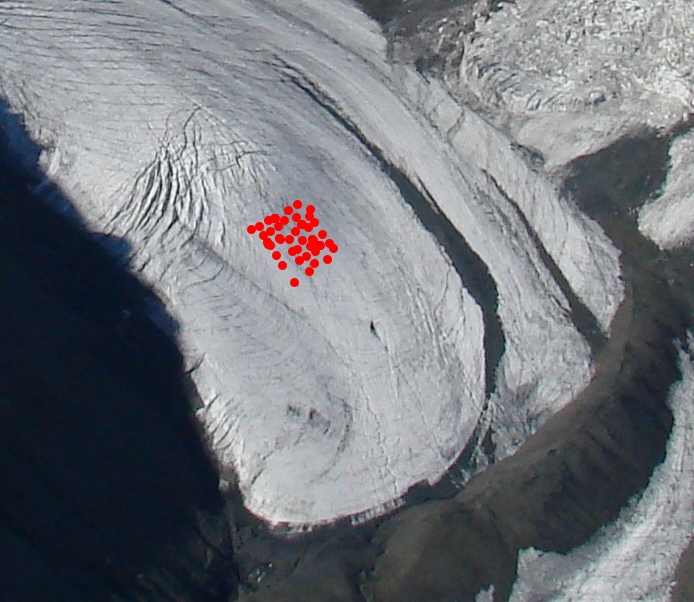
\includegraphics[width=5cm,height=4.5cm]{probe_cell.jpeg}
  \subcaption{Grid}
  \par\vfill
  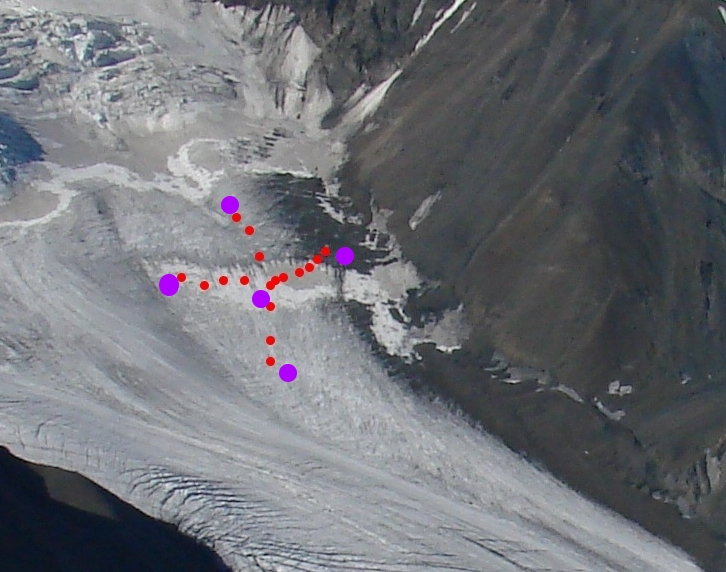
\includegraphics[width=5cm,height=4.5cm]{probe_curvature.jpeg}
  \subcaption{Cross Transect}
\end{minipage}%
\begin{minipage}[c][11cm][t]{.33\textwidth}
	\vspace*{\fill}
  \centering
  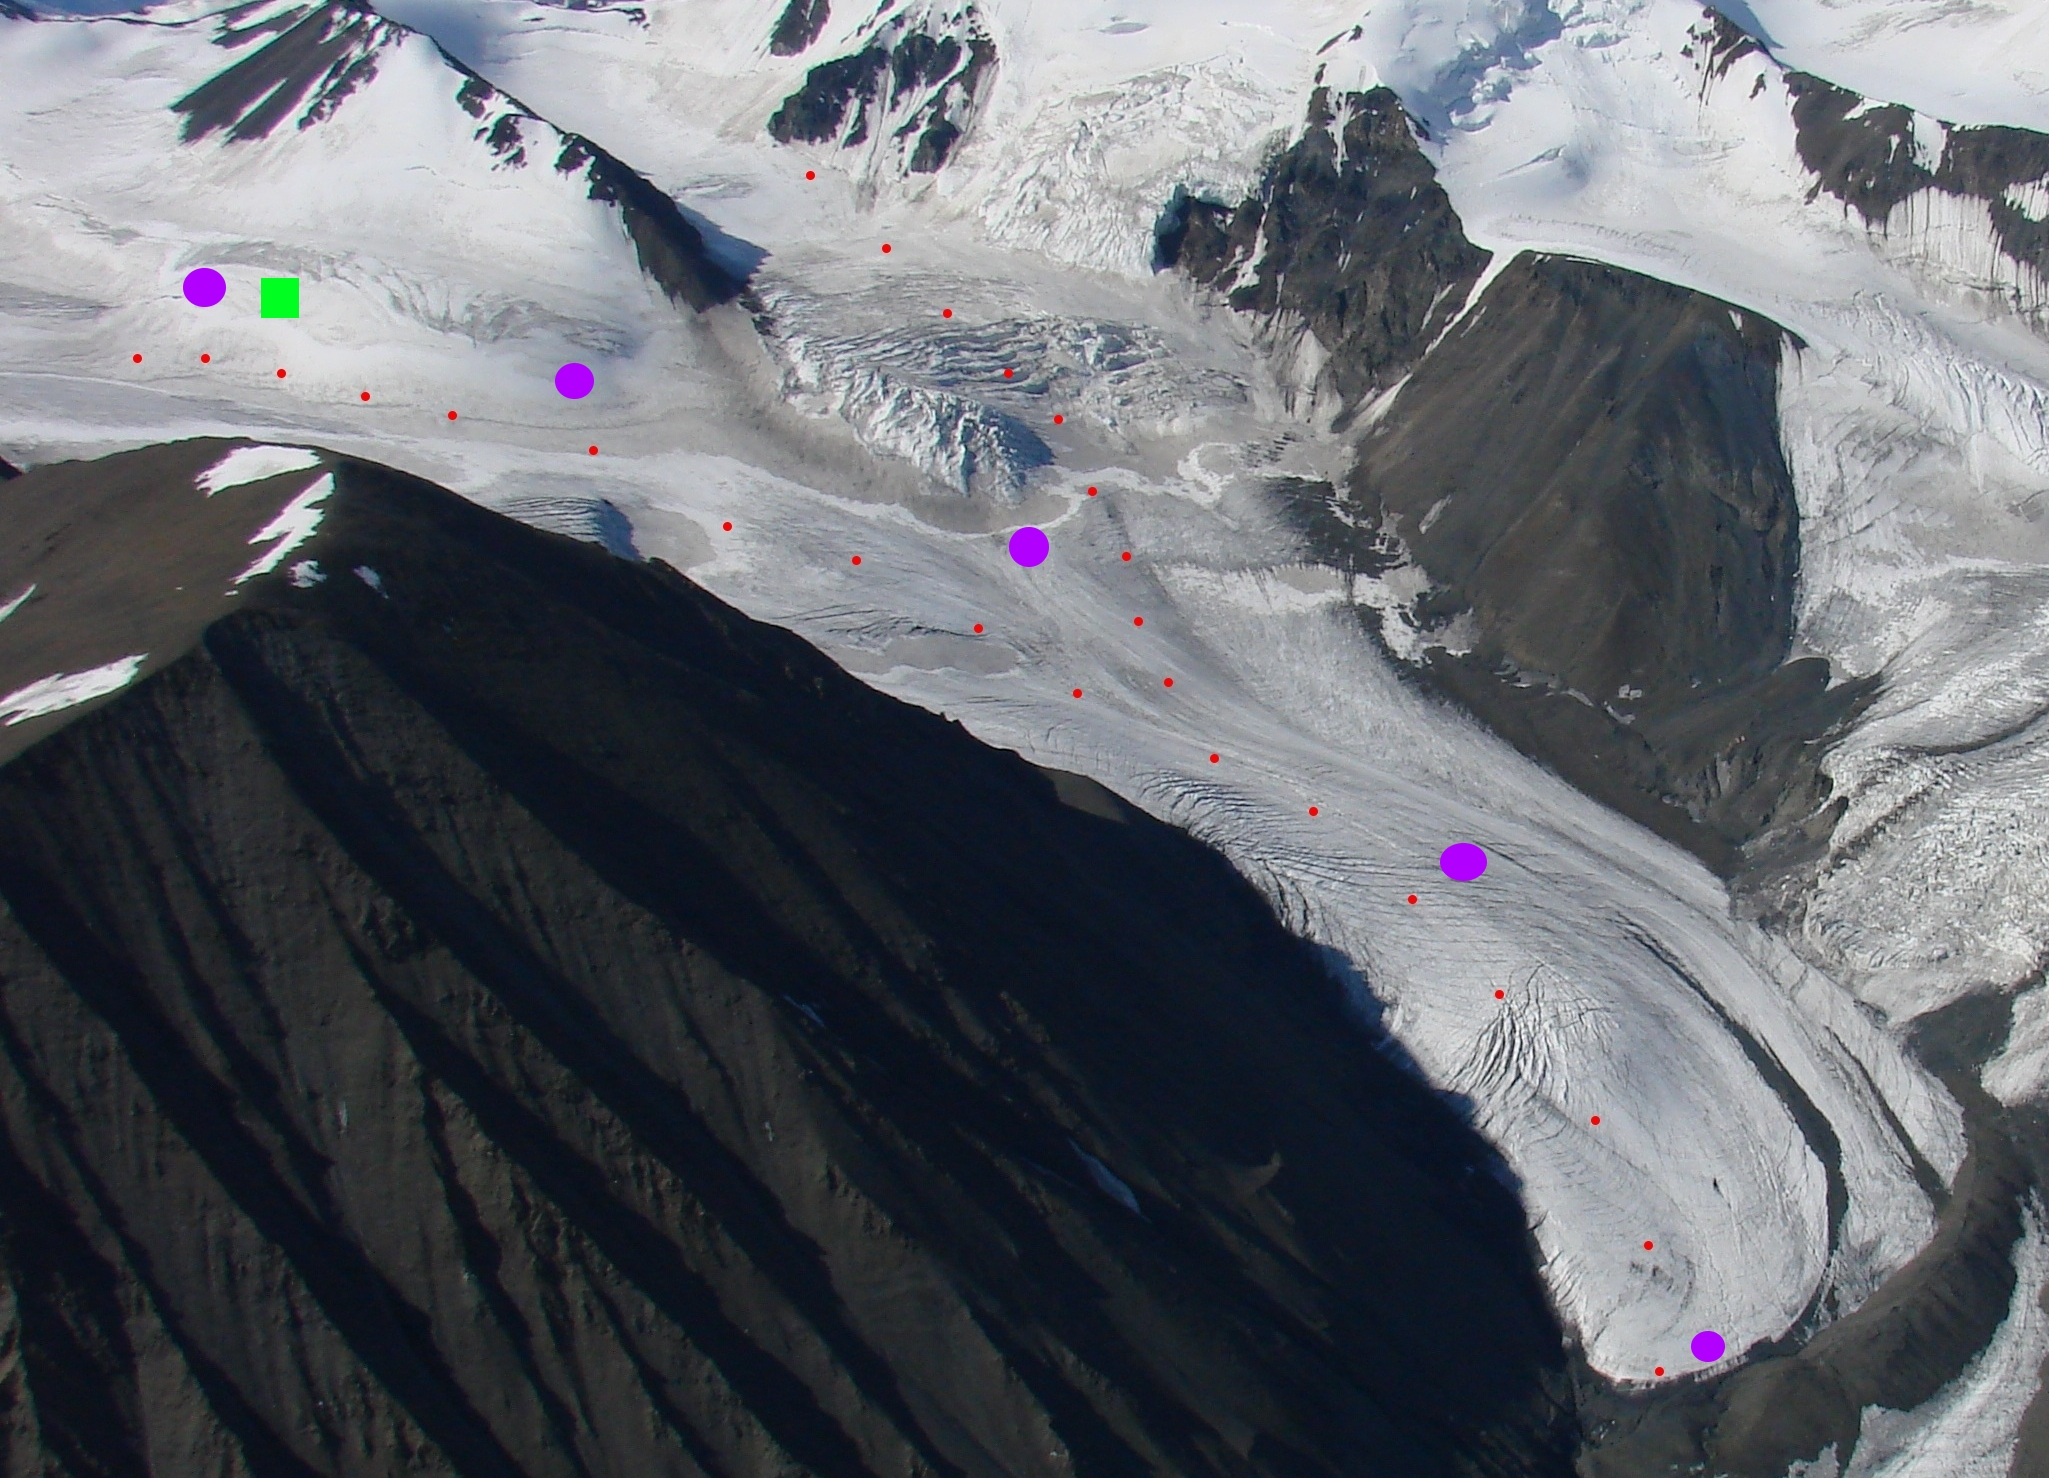
\includegraphics[width=5cm,height=4.5cm]{probe_transect.jpeg}
  \subcaption{Centre line transect}
\par\vfill
  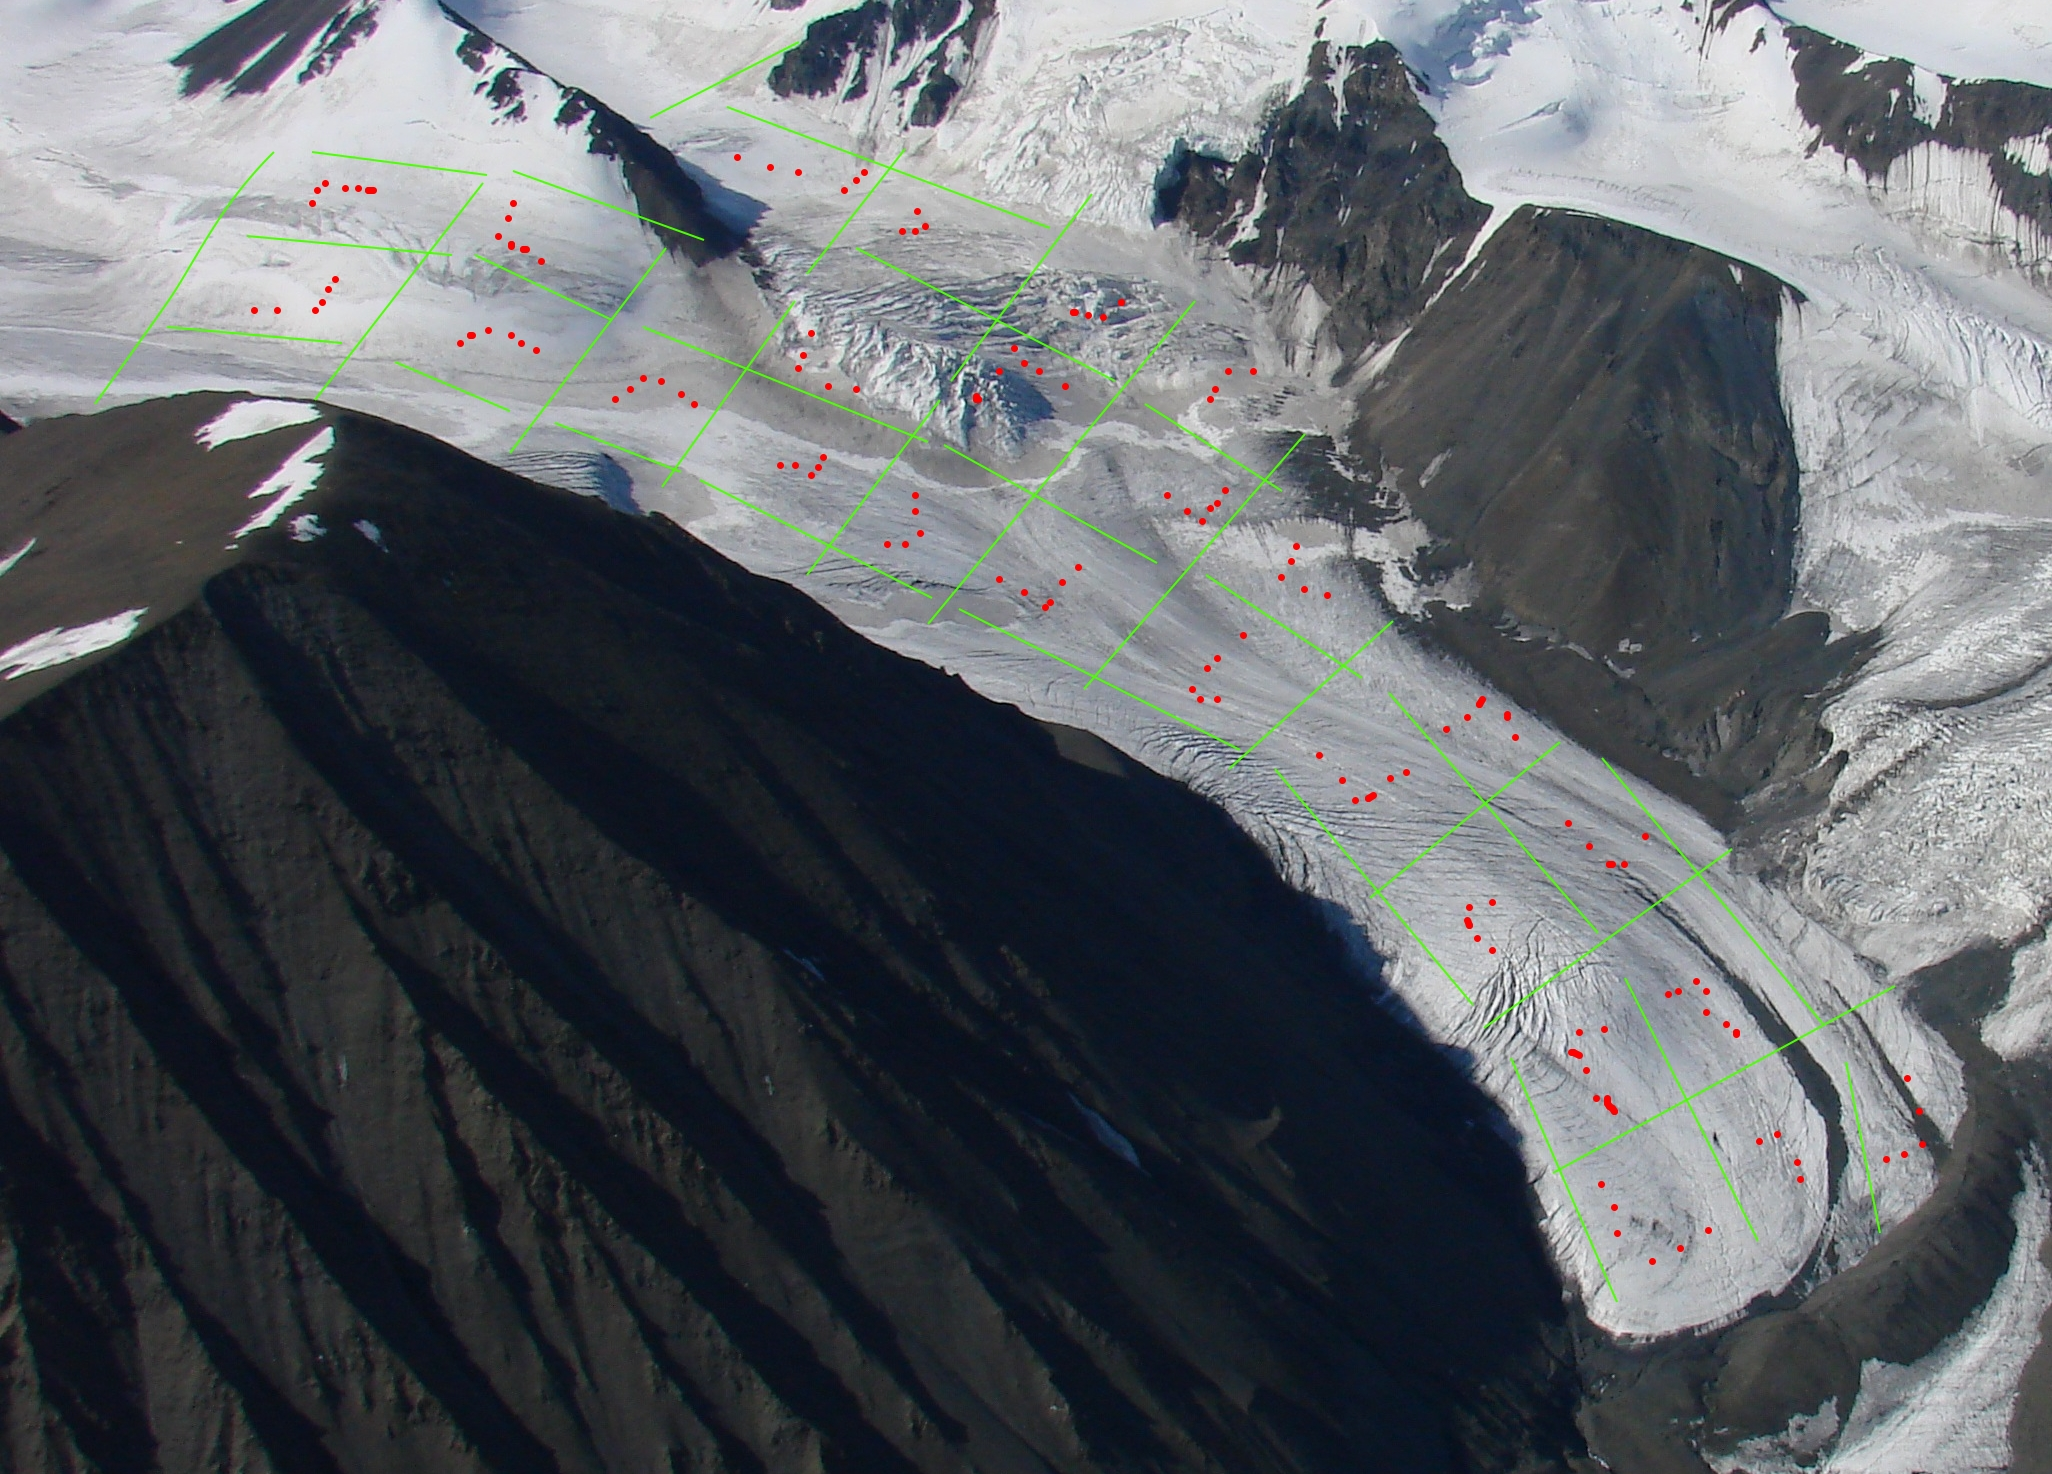
\includegraphics[width=5cm,height=4.5cm]{probe_L.jpeg}
  \subcaption{``L'' in Grid}
\end{minipage}%
\begin{minipage}[c][11cm][t]{.33\textwidth}
	\vspace*{\fill}
  \centering
    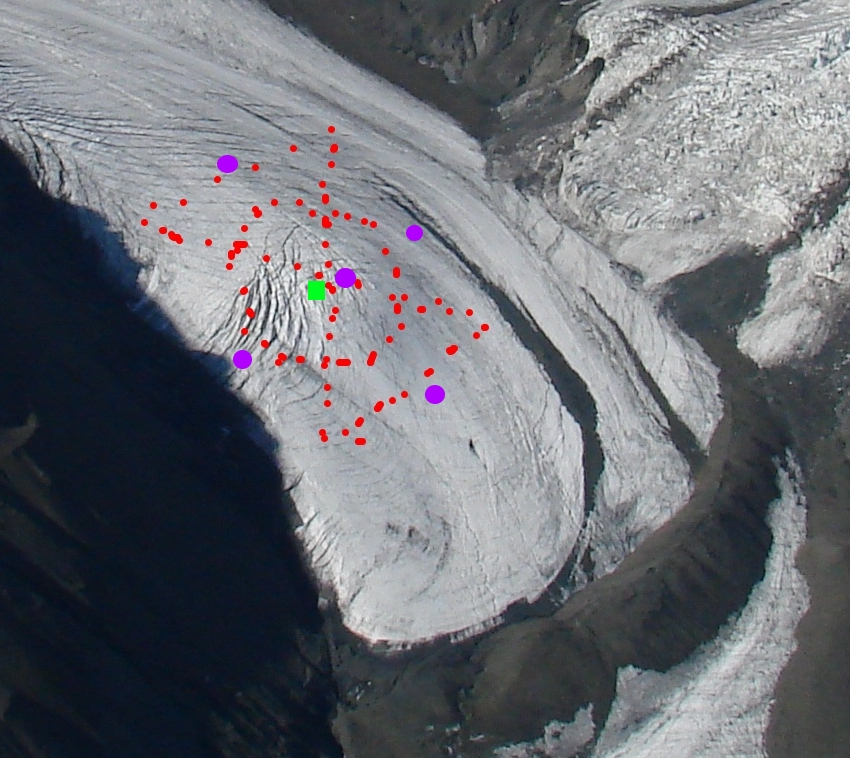
\includegraphics[width=5cm,height=4.5cm]{probe_hourglass.jpeg}
  \subcaption{Hourglass with circle}
   \par\vfill
   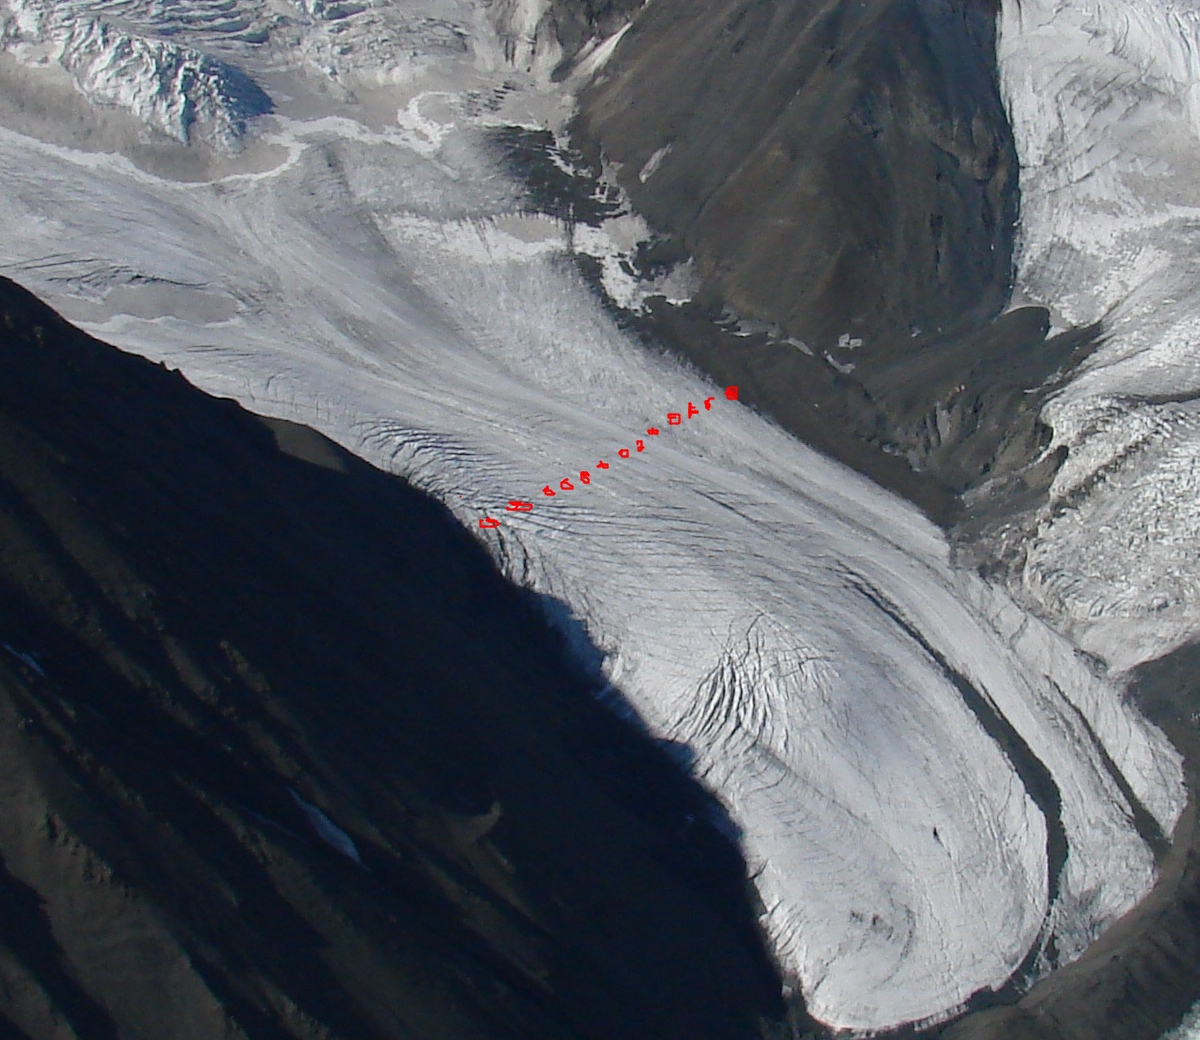
\includegraphics[width=5cm,height=4.5cm]{probe_transverse.jpeg}
  \subcaption{Transverse transect}
\end{minipage}

\caption{Examples of proposed sampling patterns. See Table \ref{fieldplan} for more details. Probing lines are shown as dotted red lines, firn cores as a purple circles, and snow pits as a green squares.}
\label{glacier}
\end{figure}


\begin{table}[]
\centering
\caption{Tentative combinations of sampling patterns and the number of locations they will be completed for each of the three or four study glaciers. 'Reps' means the number of times each set of probing, snow cores, and snow pits will be done on each glacier.}
\label{my-label}
\begin{tabular}{cc|lccc|c}
                                                                                          &                                  &                          & \textbf{Probing}                                                                                          & \textbf{Snow Cores}       & \textbf{Snow Pits}        & \textbf{Reps}             \\ \hline
\multicolumn{1}{l}{}                                                                      & \multicolumn{1}{l|}{}            &                          & \multicolumn{1}{l}{}                                                                                      & \multicolumn{1}{l}{}      & \multicolumn{1}{l|}{}     & \multicolumn{1}{l}{}      \\
\rowcolor[HTML]{EFEFEF} 
\cellcolor[HTML]{EFEFEF}                                                                  & Ablation                         &                          & \begin{tabular}[c]{@{}c@{}}Grid + Hourglass \\ + Transverse transect\end{tabular}                         & 5                         & 1                         & 4                         \\
\multirow{-2}{*}{\cellcolor[HTML]{EFEFEF}\textbf{Glacier A}}                              & Full                             &                          & \begin{tabular}[c]{@{}c@{}}Centre line transect, \\ ``L'' in grid\end{tabular}                            & 5, every cell             & 3 (for both)              & 1                         \\
                                                                                          & \cellcolor[HTML]{EFEFEF}Ablation & \cellcolor[HTML]{EFEFEF} & \cellcolor[HTML]{EFEFEF}\begin{tabular}[c]{@{}c@{}}Grid + Hourglass \\ + Transverse transect\end{tabular} & \cellcolor[HTML]{EFEFEF}5 & \cellcolor[HTML]{EFEFEF}1 & \cellcolor[HTML]{EFEFEF}2 \\
\multirow{-2}{*}{\textbf{\begin{tabular}[c]{@{}c@{}}Glaciers \\ B, C, (D?)\end{tabular}}} & Full                             &                          & \begin{tabular}[c]{@{}c@{}}Centre line transect, \\ ``L'' in grid\end{tabular}                            & 5, every cell             & 2                         & 1                         \\
\rowcolor[HTML]{EFEFEF} 
\multicolumn{2}{c|}{\cellcolor[HTML]{EFEFEF}}                                                                                &                          & \begin{tabular}[c]{@{}c@{}}Dense transect (drift, \\ accumulation, ablation)\end{tabular}                 & 3                         & 0                         & 1                         \\
\multicolumn{2}{c|}{\multirow{-2}{*}{\cellcolor[HTML]{EFEFEF}\textbf{Where present}}}                                        &                          & \begin{tabular}[c]{@{}c@{}}Cross transect \\ (high curvature)\end{tabular}                                & 5                         & 0                         & 1-2                      
\end{tabular}
\end{table}

The proposed research aims to examine the spatial and temporal variability of snow in the St. Elias Mountains using direct measurements and statistical models. The spatial variability will be measured by conducting an extensive snow survey in May 2016. Accumulation will be measured using a combination of probing, firn coring, and snow pits on three to four alpine glaciers in the Donjek Range, located in the eastern part of the St. Elias Mountains. Integrated snow density will be determined by drilling firn cores and weighing them. Density is known to vary less than snow depth so far fewer firn cores will be extracted \citep{Ostrem1991}. Each glacier will have a minimum of three snow pits --- one in the ablation zone, one near the equilibrium line altitude, and one in the accumulation area --- and at least five cores, as seen in Figure \ref{glacier}. If snow drifts are found then the firn corer can also be used to examine variation in snow density perpendicular to the drifts. 

Probing will be done at point, hillslope, and watershed scales in a number of patterns and orientations, as seen in Table \ref{fieldplan} and Figure \ref{glacier}, in an attempt to quantify variability at multiple scales. Transects at both the point and watershed scales can be used to generate variograms, which provide insight into length scales of relevant process \citep[e.g.][]{Goovaerts2000}. The grid pattern can be used to quantify variability in accumulation within one digital elevation model (DEM) cell, which is important when considering geographical parameters calculated from DEMs. At the hillslope scale, the effect of curvature and slope can be investigated by conducting transects along areas with high curvature and nearby areas that have low curvature. At the watershed scale, the winter balance of the study glaciers will be calculated using the centre line transect as well as the ``L'' in grid pattern. The centre line transect is commonly used on glaciers \citep[e.g.][]{Ostrem1991} but is only able to capture accumulation changes along the elevation gradient. The ``L'' in grid pattern \citep[see][for more details]{Elder2009} allows for the whole study area to be represented and aims to minimize bias by randomizing the orientation, location, and resolution of transects at right angles. A comparison of the winter balance found with these two methods could be used to optimize future glacier snow surveys. The hourglass with circle pattern can be applied at any scale. Its main advantage is that it captures accumulation measurements in many directions but is also able to cover a large area. Since it requires dense probing, it will only be done in the ablation zone, where the previous summer surface is well-defined.

Measured accumulation at these scales will be related to geographic parameters, as seen in Figure \ref{flow_geography}. Geographic parameters will be calculated from SPOT5 DEMs (40 x 40 m resolution) or ASTER GDEM (30 m posting and 1 x 1 degree tiles). Both linear statistical methods (e.g. multiple linear regression) and non-linear methods (e.g. regression tree models) will be applied to best try to capture the relationships between geography and accumulation.

\begin{figure*}[t!]
    \begin{subfigure}[t]{0.5\textwidth}
        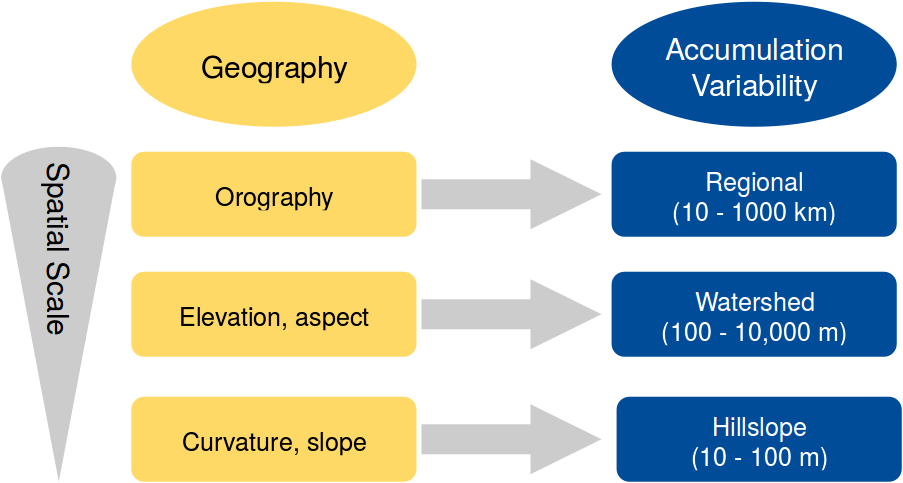
\includegraphics[height=1.7in]{flow_geography.png}
        \caption{}
        \label{flow_geography}
    \end{subfigure}%
    ~
    \begin{subfigure}[t]{0.5\textwidth}
    	\raisebox{0.12\textwidth}{%   	
        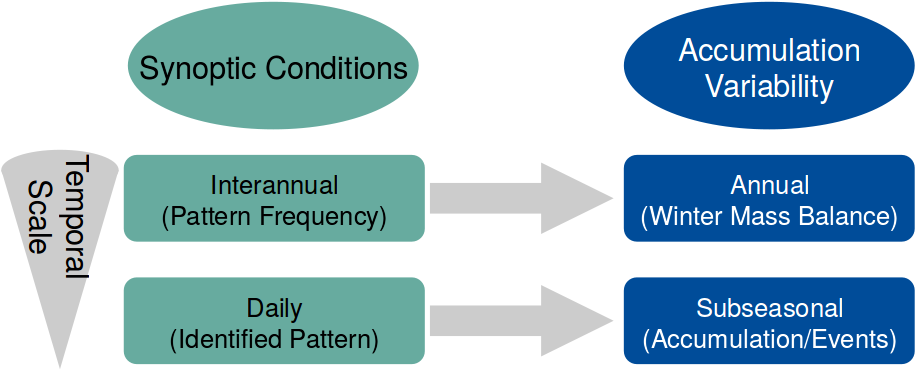
\includegraphics[height=1.3in]{flow_synoptic.png}}
        \caption{}
        \label{flow_synoptic}
    \end{subfigure}
    \caption{Proposed statistical relationships (arrows) between geography (a) and accumulation variability and synoptic conditions (b) and accumulation variability at various scales. Scales of `Accumulation variability' taken from \cite{Clark2011}.}
\end{figure*}

The three to four study glaciers (Glacier A, B, C, and maybe D) have yet to be confirmed but an image of the proposed study sites can be seen in Figure \ref{donjek}. To compare accumulation at the regional scale, various orientations and locations of glaciers were chosen. Glaciers with opposite orientations were chosen to investigate potential effects of solar radiation on SWE. Additionally, anecdotal observations indicate that storms usually track either from the north or the south of the Donjek Range. Furthermore, the glaciers on the SE side of the range seem to receive greater accumulation, which may indicate a range crest that divides the NW and SE parts of the range (Flowers, 2016, personal communication). Glaciers in the SW and NE areas were chosen to investigate the possible effects of distance from the moisture source (predominantly northern Pacific Ocean) and from the topographic divide, which is located west of the Kaskawalsh Glacier \citep{Taylor1969}. Of the glaciers in the Donjek Range, only medium-sized alpine glaciers were considered and any that were dangerous due to heavy crevassing were excluded. Figure \ref{donjek} (a) shows potential study glaciers in the Donjek Range. The exact glaciers will be chosen by further study of satellite and DEM imagery prior to the field season.  

\begin{figure}
\begin{minipage}[c][20cm][t]{.5\textwidth}
	\vspace*{\fill}
  \centering
  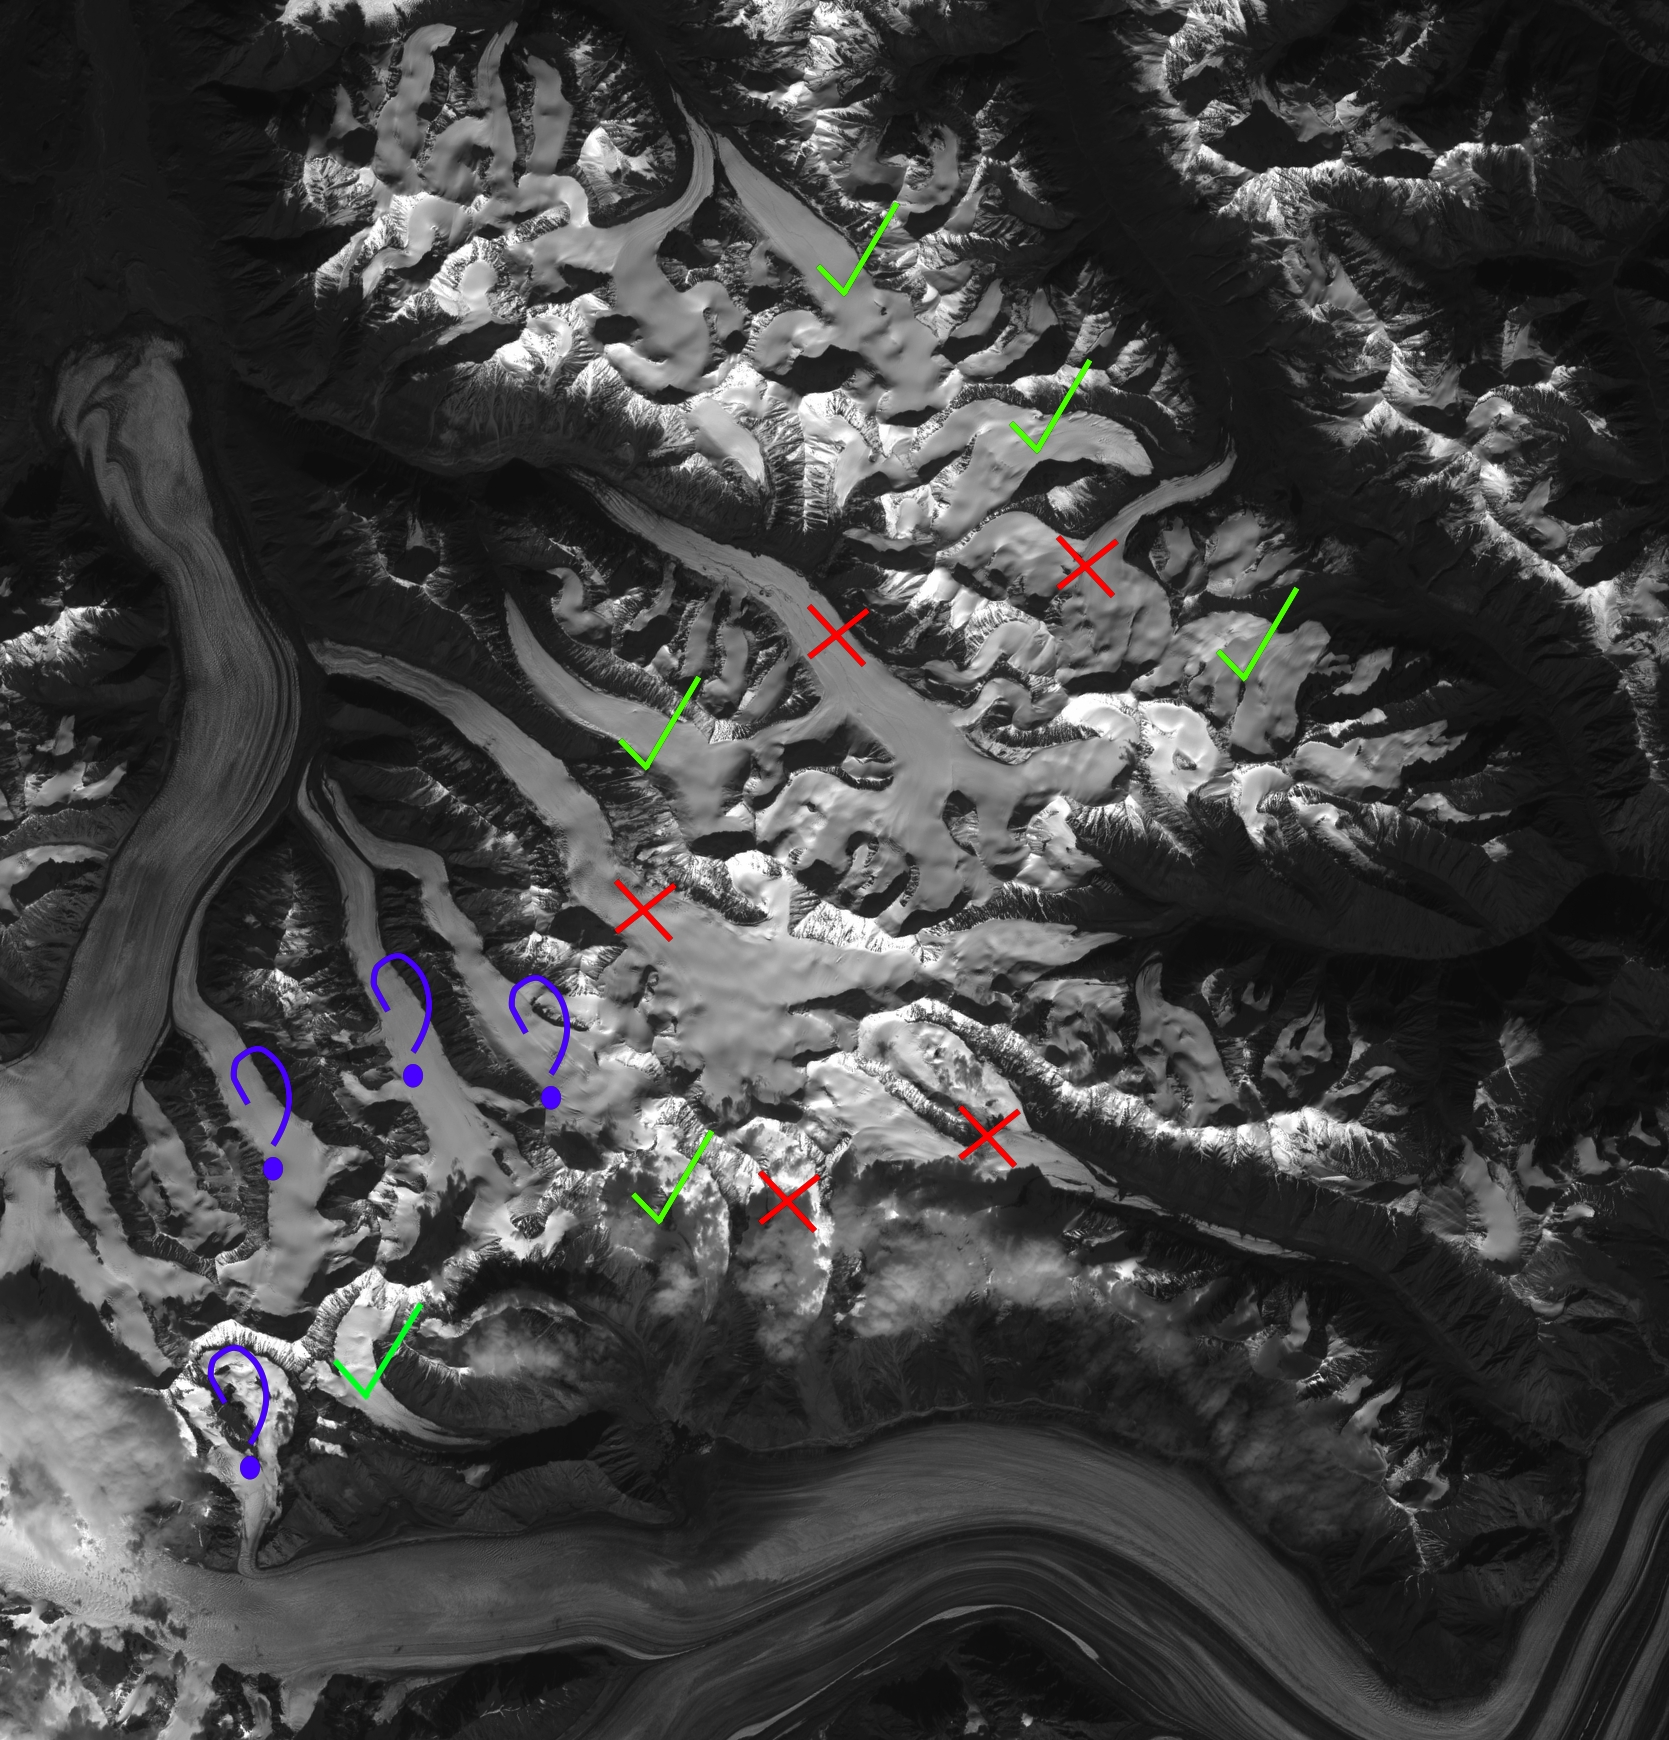
\includegraphics[width=0.95\textwidth]{donjeck_x.jpg}
  \subcaption{Glacier accessibility. Red `X's are placed on glaciers that are too dangerous, green check marks are placed on glaciers that are known to be safe, and purple question marks are places on glaciers that have not yet been observed so their safety cannot be confirmed.}
  \par\vfill
  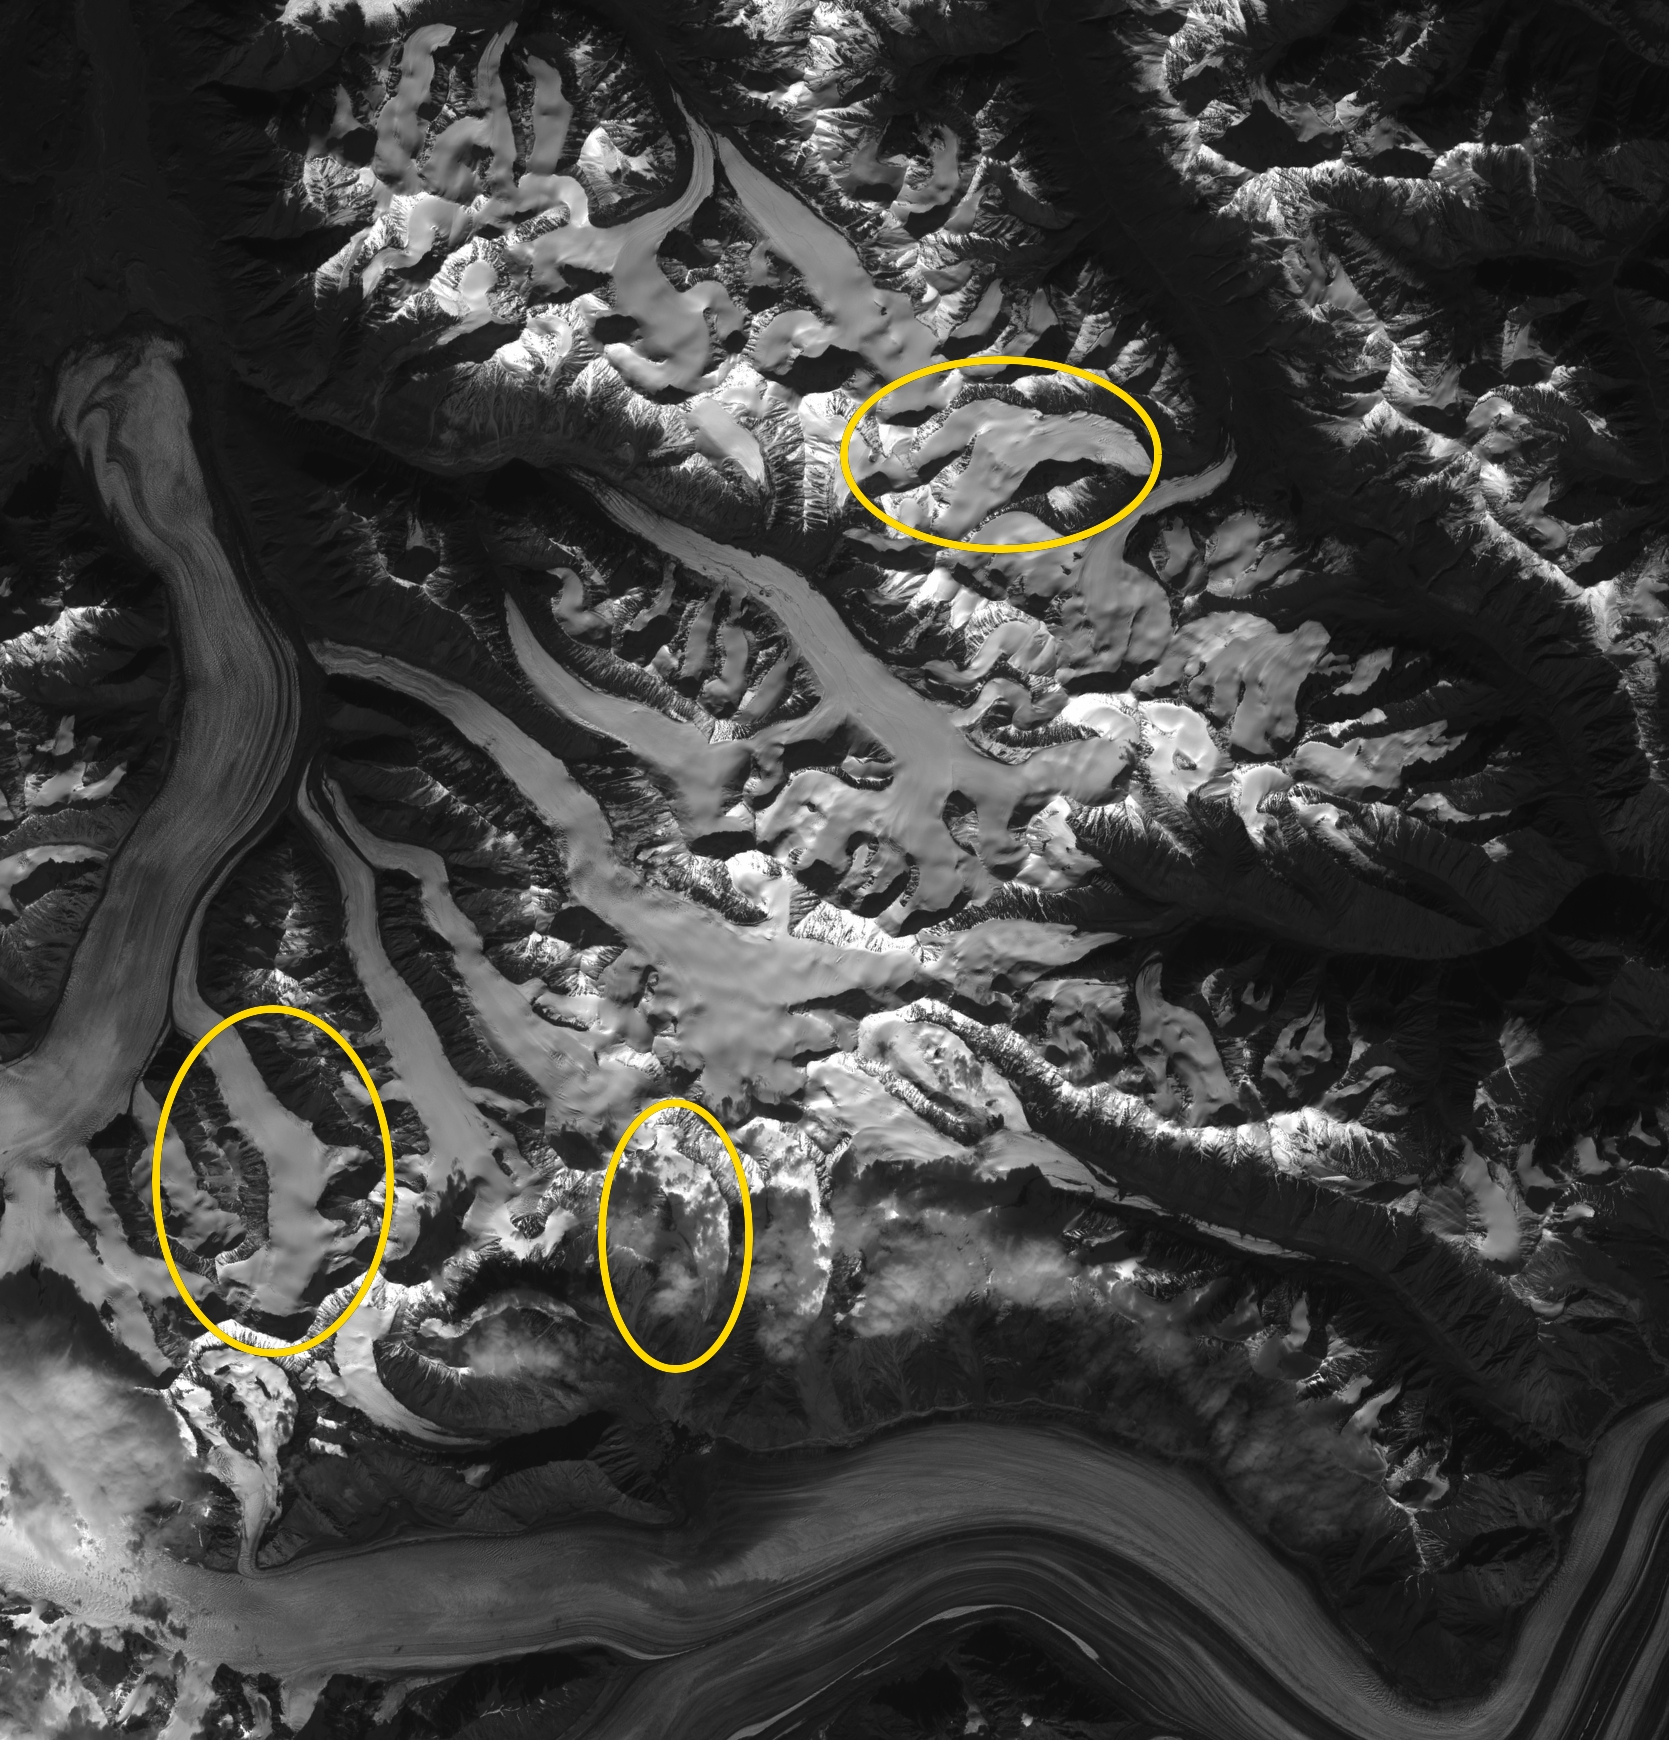
\includegraphics[width=0.95\textwidth]{donjeck_1.jpg}
  \subcaption{Proposed study glacier set 1}
\end{minipage}%
\begin{minipage}[c][20cm][t]{.5\textwidth}
	\vspace*{\fill}
  \centering
  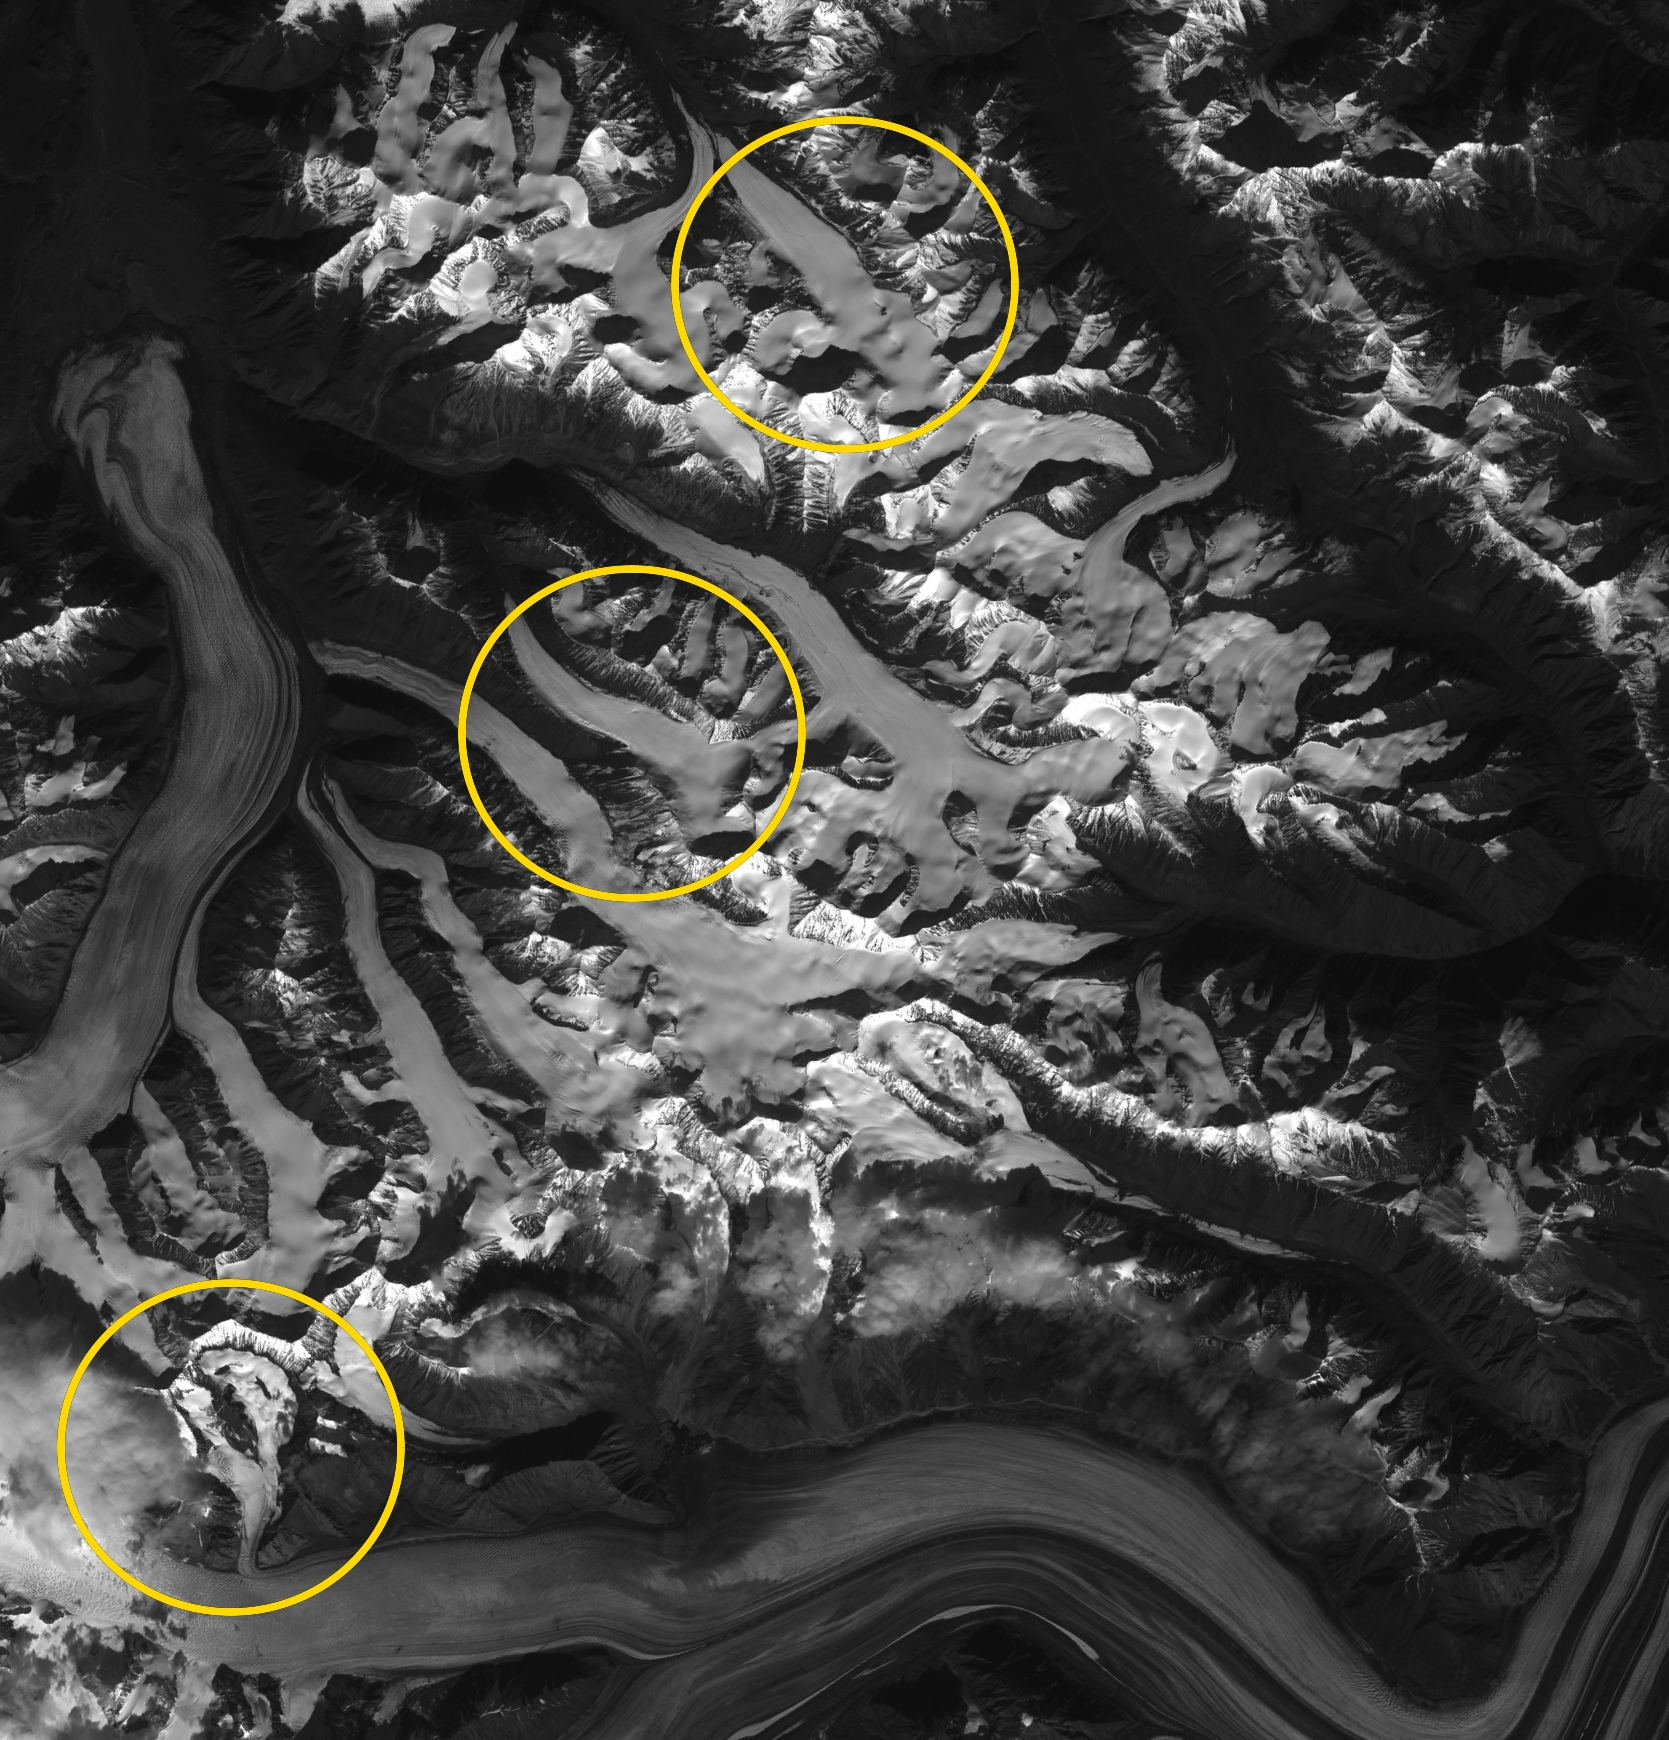
\includegraphics[width=0.95\textwidth]{donjeck_2.jpg}
  \subcaption{Proposed study glacier set 2}
  \par\vfill
  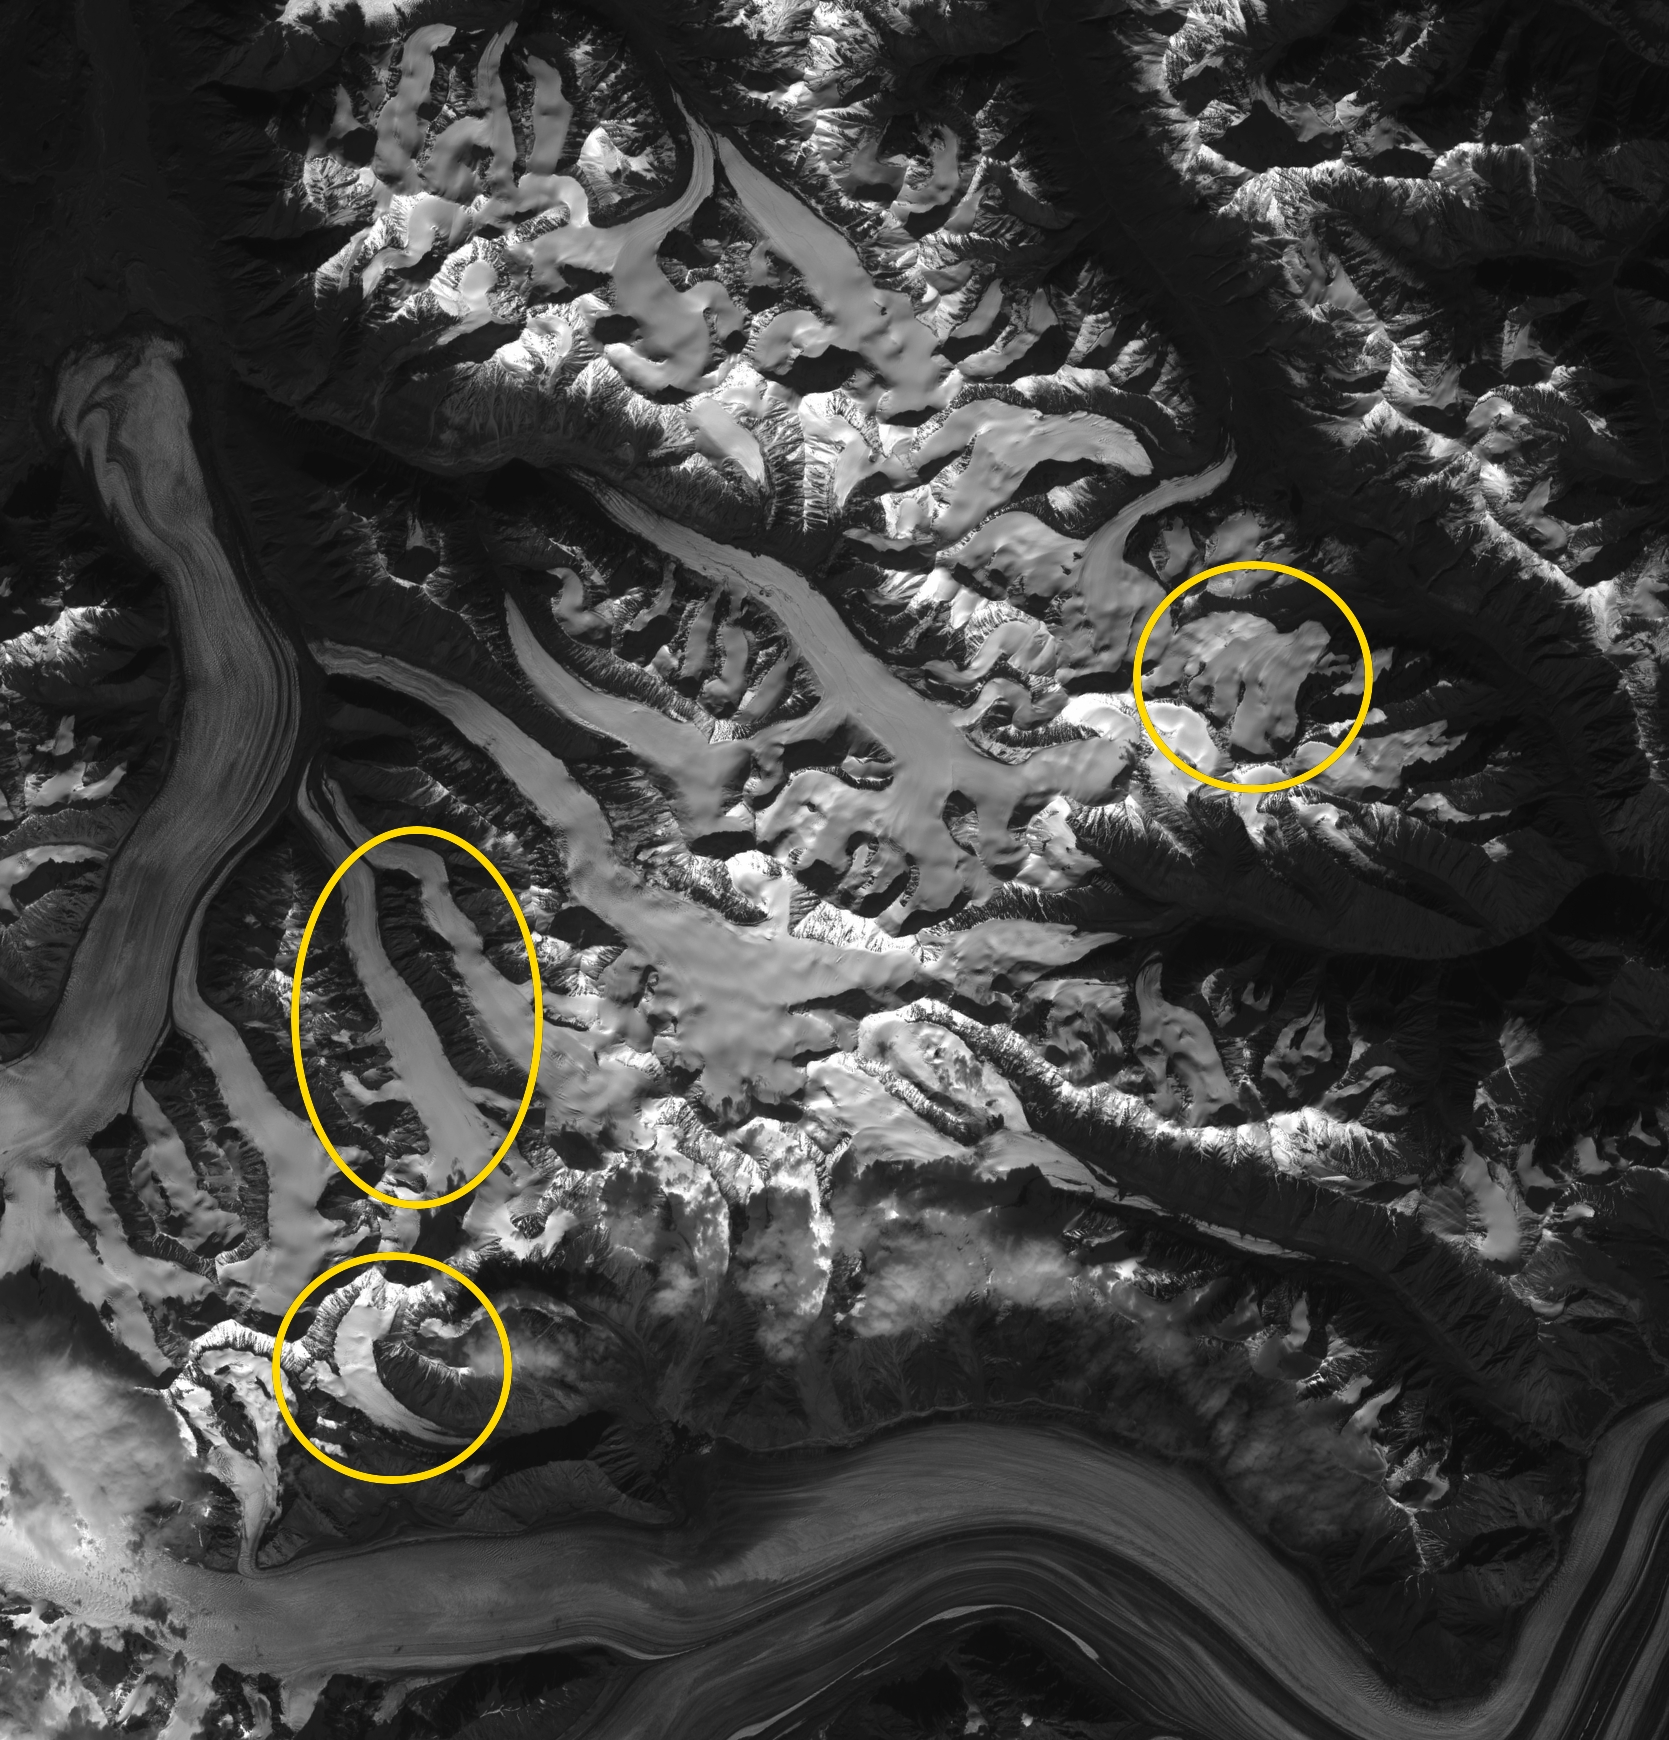
\includegraphics[width=0.95\textwidth]{donjeck_3.jpg}
  \subcaption{Proposed study glacier set 3}
\end{minipage}%

\caption{Considered study glaciers in the Donjek Range}
\label{donjek}
\end{figure}

To examine temporal variability, previously collected accumulation data will be used. Accumulation estimates from snow pit and depth probing measurements conducted in earlier campaigns (2007--09 and 2011--14) on two alpine glaciers (South and North Glaciers) in the Donjek Range will be correlated with the occurrence of synoptic weather patterns. Weather conditions in the North Pacific will be obtained from ERA-Interim reanalysis data and statistical methods, including PCA and neural networks, will then be applied to find weather patterns. Similar statistical methods will be applied to relate subseasonal accumulation, recorded with an SR50 from 2012--14, to  patterns identified in the synoptic conditions. These relationships are shown in Figure \ref{flow_synoptic}. 

Preliminary work to correlate synoptic patterns to glacier-wide accumulation reveals significant correlations between patterns in the 750 hPa geopotential, found using a self organizing map (SOM), and winter balance between 2007 and 2011. This indicates that accumulation is likely to be affected by interannual variability in large-scale atmospheric circulation. However, further investigation is needed because the original analysis used winter accumulation determined from a regression model for five study years --- using this small number of values that contain their own extrapolation errors limits the strength of the conclusions. Correlations with direct SWE measurements would likely provide a more accurate interpretation of relationships between synoptic conditions and glacier accumulation. It would also be valuable to examine subseasonal accumulation from winter SR50 records because those records allow for a higher temporal resolution of accumulation data, and thus more points that can be used in the correlation. 

\section{Summary}
The contribution of accumulation to glacier mass balance is controlled mainly by the distribution of snow. Processes such as orographic lifting, preferential deposition, and wind redistribution, all arising from the interaction of atmospheric conditions and topography, strongly affect snow distribution. Statistical models have been used to relate meteorological and topographic variables to snow accumulation in order to better understand the effects of these processes. These models rely on accurate measurement of snow distribution, which can be achieved by determining SWE from snow density and depth. Results from previous studies of accumulation on glaciers have shown large spatial variability at many scales and a dependence on multiple processes that affect snow distribution. Accumulation in the St. Elias Mountains is poorly understood, largely because the glaciers are remote. There is therefore a need to quantify snow accumulation in this region and how it varies both between glaciers and within glacierized basins. The proposed study would be the first within the St. Elias Mountains to examine inter- and intra-basin accumulation variability. Well-established methods would be applied to measure accumulation variability, which would then be statistically correlated with geographical and synoptic parameters. This study will provide valuable insight into the variability of snow on glaciers at various scales and the processes and conditions that affect variability. 

\pagebreak
\bibliography{/home/glaciology1/Documents/MastersLit}
\bibliographystyle{igs}
\end{document}
